\documentclass[aspectratio=169,11pt]{beamer}

% Theme
\usetheme{Madrid}
\usecolortheme{default}
\setbeamertemplate{navigation symbols}{}
\setbeamertemplate{footline}[frame number]
\setbeamertemplate{caption}{\raggedright\insertcaption\par} % no "Figure:" prefix

% Packages
\usepackage[utf8]{inputenc}
\usepackage[T1]{fontenc}
\usepackage{graphicx}
\usepackage{booktabs}
\usepackage{amsmath,amssymb}
\usepackage{xcolor}
\usepackage{microtype}

% Paths
\graphicspath{{../results/}{../docs/}}

% Colors
\definecolor{polimi}{RGB}{0,45,100}
\definecolor{fcosblue}{RGB}{33,150,243}
\definecolor{retinaorange}{RGB}{255,152,0}
\definecolor{fastergreen}{RGB}{76,175,80}
\definecolor{good}{RGB}{27,120,55}
\definecolor{bad}{RGB}{178,24,43}

\setbeamercolor{structure}{fg=polimi}
\setbeamercolor{title}{fg=white,bg=polimi}
\setbeamercolor{frametitle}{fg=white,bg=polimi}
\setbeamerfont{frametitle}{series=\bfseries}

% Compact itemize
\setbeamertemplate{itemize items}[circle]
\newcommand{\hl}[1]{\textcolor{polimi}{\textbf{#1}}}

%==============================================================================
\title[Anchor-Free vs.\ Anchor-Based Pneumonia Detection]{Pneumonia Detection Using\\ Anchor-Free vs.\ Anchor-Based Object Detection}
\subtitle{Reproducing and Extending Wu et al.\ (2024)}
\author[Mandour \& Nuttini]{Mohamed Z.\ M.\ Mandour \and Elena Nuttini}
\institute[PoliMI]{Numerical Analysis for Machine Learning\\Politecnico di Milano}
\date{June 2026}
\titlegraphic{
\includegraphics[height=1.4cm]{logo_polimi.png}}

\begin{document}

%------------------------------------------------------------------------------
\begin{frame}[plain]
  \titlepage
\end{frame}

%------------------------------------------------------------------------------
\begin{frame}{Outline}
  \small
  \begin{columns}[t]
    \column{0.5\textwidth}
      \begin{enumerate}\setlength\itemsep{0.4em}
        \item Problem \& dataset
        \item The reference paper \& our question
        \item Detection paradigms \& models
        \item Training recipe \& numerical analysis
      \end{enumerate}
    \column{0.5\textwidth}
      \begin{enumerate}\setlength\itemsep{0.4em}\setcounter{enumi}{4}
        \item Metrics
        \item Results \& the honest paper comparison
        \item Calibration artefact \& robustness
        \item Limitations \& conclusion
      \end{enumerate}
  \end{columns}
  \vfill
  \footnotesize\textit{Take-home message: the contribution is \hl{methodological}, a fair,
  statistically honest comparison, not a new state-of-the-art model.}
\end{frame}

%------------------------------------------------------------------------------
\begin{frame}{Problem \& Dataset}
  \begin{columns}[T]
    \column{0.58\textwidth}
      \textbf{Task: object detection, not classification}
      \begin{itemize}\small
        \item Not ``is there pneumonia?'' but \hl{where}, predict bounding boxes + confidence.
        \item Opacities are subtle, variable in shape, overlapping.
      \end{itemize}
      \vspace{0.6em}
      \textbf{RSNA Pneumonia Detection Challenge}
      \begin{itemize}\small
        \item \hl{26{,}684} chest X-rays (DICOM), box annotations.
        \item Only \hl{$\sim$22\%} positive $\Rightarrow$ strong class imbalance.
        \item Patient-level 80/20 split (seed 42), no patient leakage.
      \end{itemize}
    \column{0.40\textwidth}
      \centering
      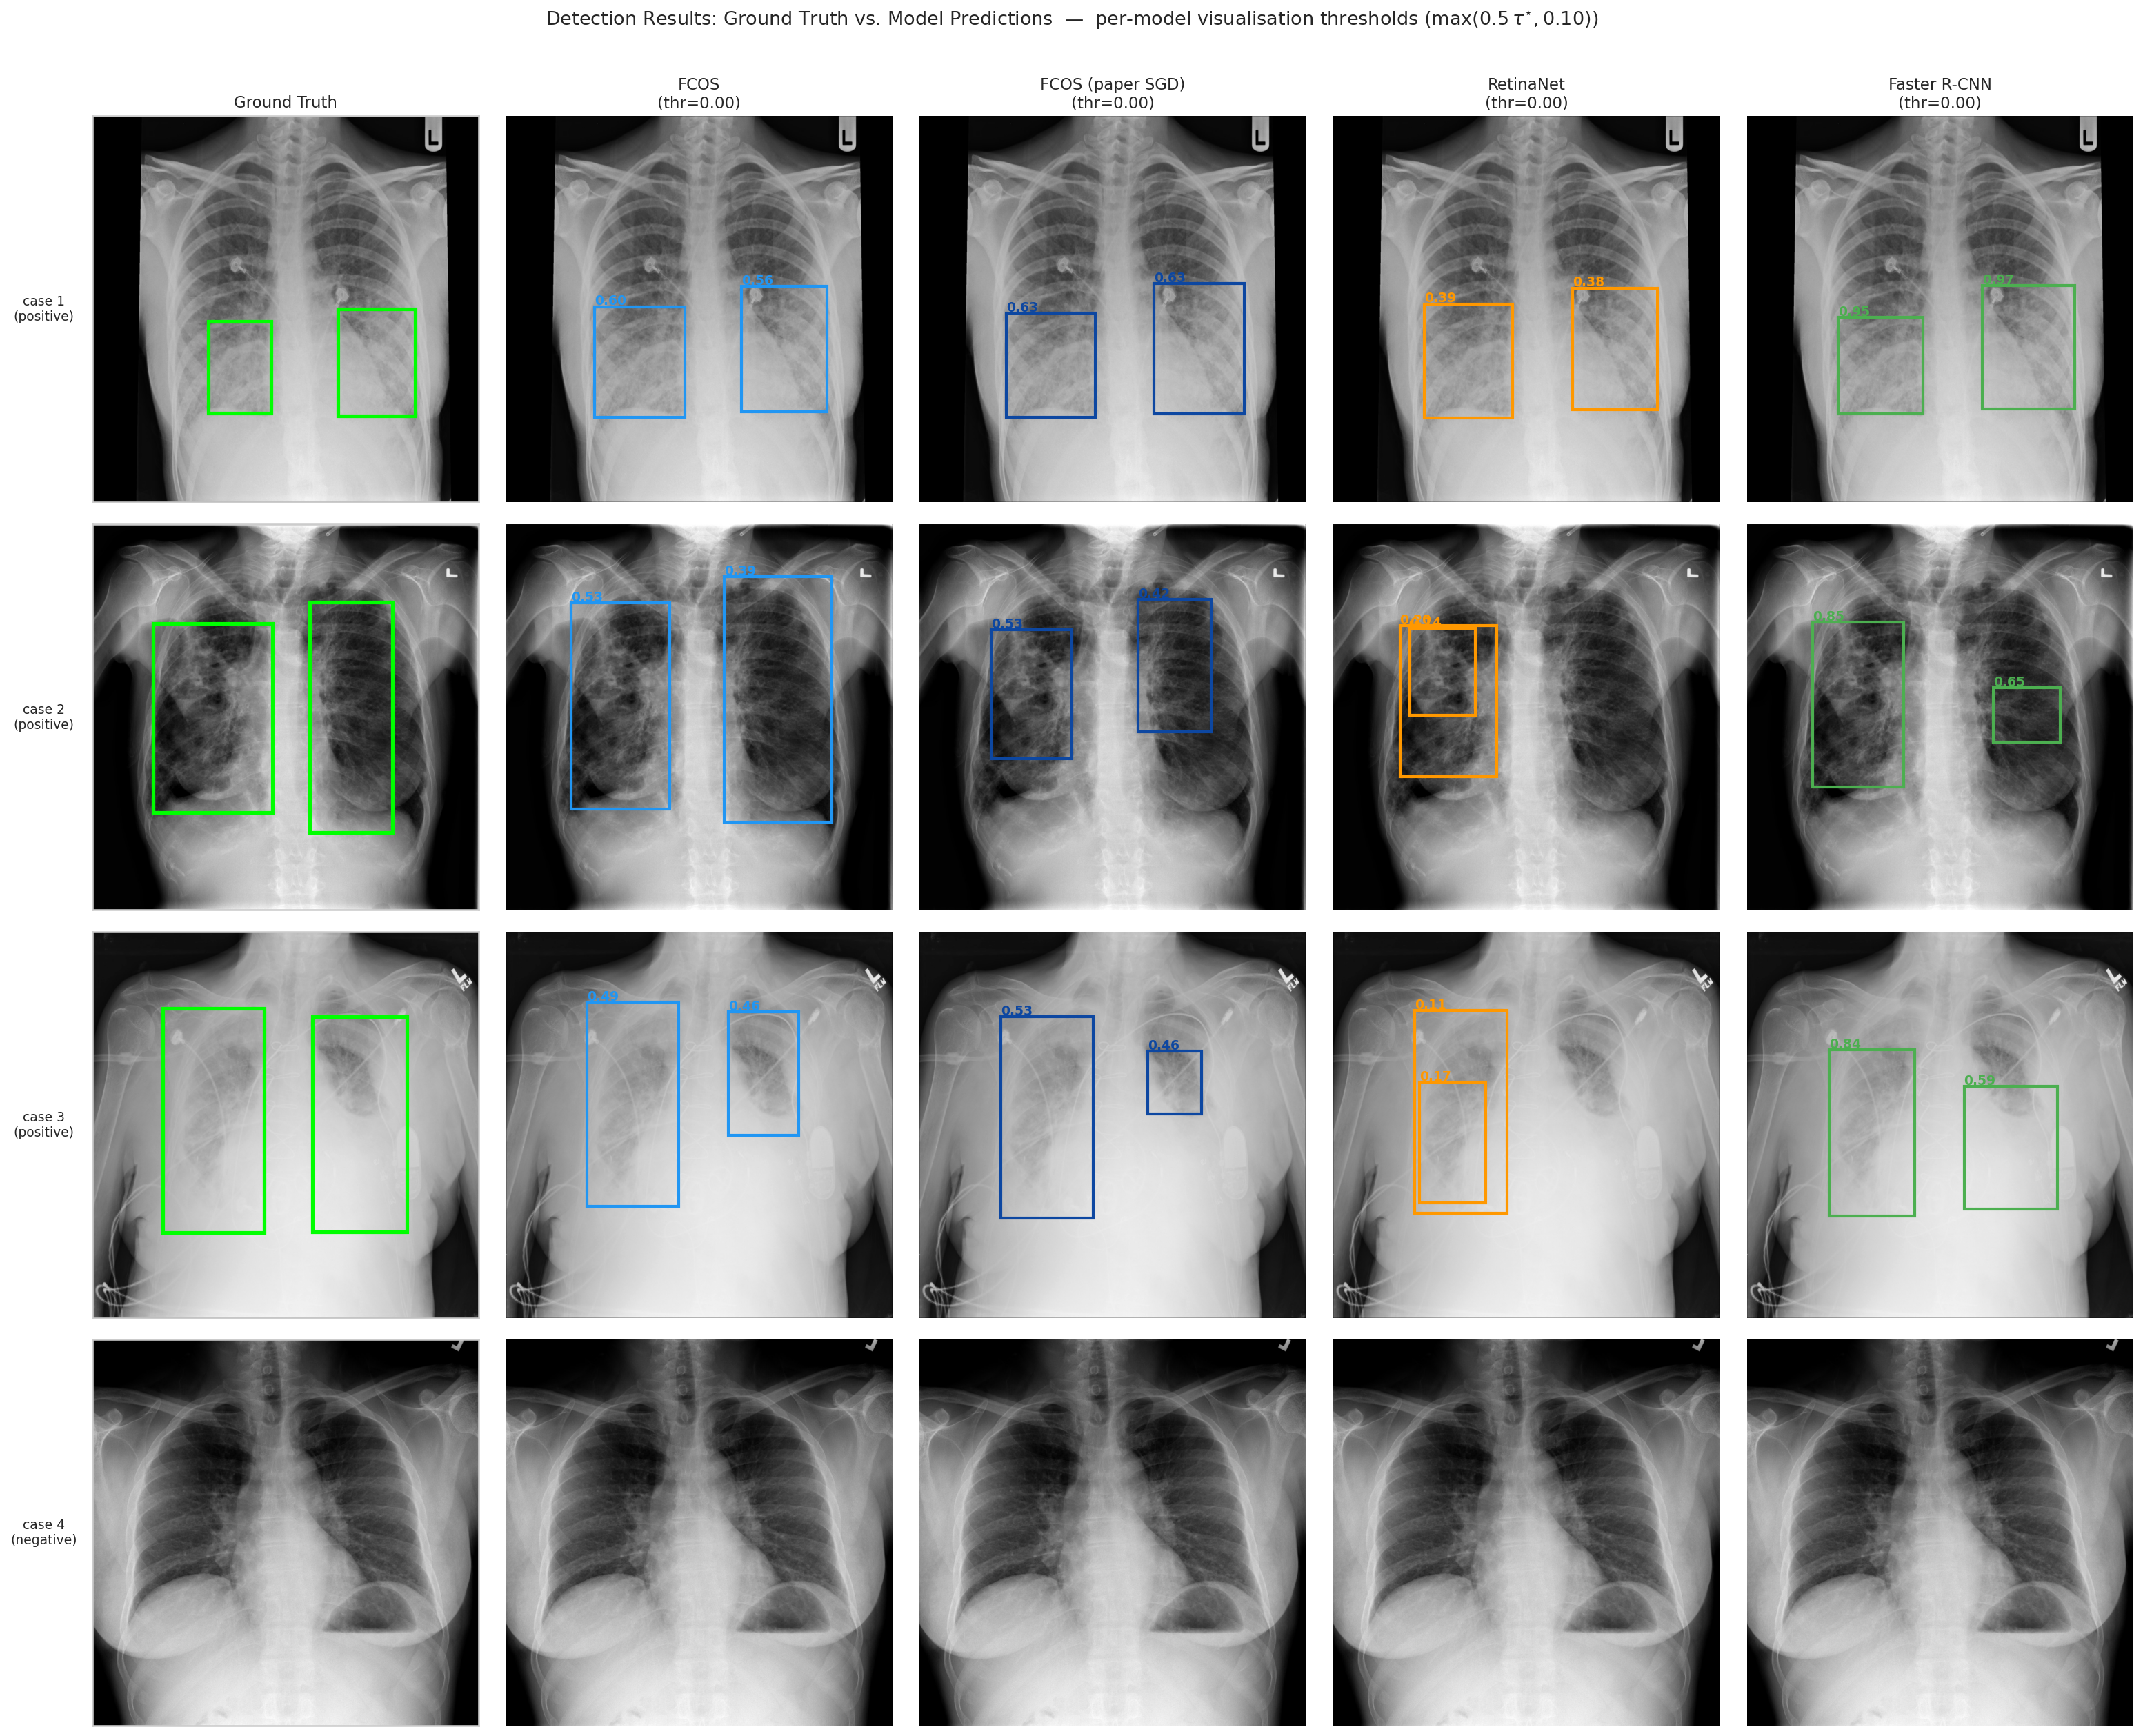
\includegraphics[height=0.62\textheight]{detection_samples.png}\\
      {\scriptsize Green = ground truth; colours = per-model predictions.}
  \end{columns}
\end{frame}

%------------------------------------------------------------------------------
\begin{frame}{The Reference Paper (Wu et al.\ 2024) \& Our Question}
  \small
  \textbf{What they did:} an \hl{anchor-free} detector (FPN + two-branch head + focal loss),
  trained with \hl{Adam} (lr $10^{-3}$, batch 1) on a single RTX 2080ti.
  \vspace{0.4em}
  \begin{columns}[T]
    \column{0.52\textwidth}
      \textbf{Their reported AP@0.5 (Table 3):}
      \begin{center}\footnotesize
      \begin{tabular}{lc}
        \toprule
        Method & AP@0.5 \\ \midrule
        SSD & 25.2 \\
        Faster R-CNN & 36.5 \\
        RetinaNet & 45.8 \\
        FCOS & 48.6 \\
        \textbf{Proposed (anchor-free)} & \textbf{51.5} \\
        \bottomrule
      \end{tabular}
      \end{center}
    \column{0.46\textwidth}
      \textbf{Their claim:} anchor-free $>$ anchor-based.
      \vspace{0.5em}
      \begin{block}{\small Our research question}
        \small But they compare against baselines run with \emph{their own} pipeline (no code
        released). \hl{At a shared backbone, recipe and evaluation, who really wins?}
      \end{block}
  \end{columns}
\end{frame}

%------------------------------------------------------------------------------
\begin{frame}{Two Paradigms, One Backbone}
  \small
  \begin{columns}[T]
    \column{0.5\textwidth}
      \textbf{\textcolor{retinaorange}{Anchor-based}}
      \begin{itemize}\small
        \item Predefined anchor boxes = a geometric prior on shapes.
        \item Classify + regress offsets from each anchor.
        \item \textbf{RetinaNet} (1-stage, focal loss), \textbf{Faster R-CNN} (2-stage, RPN + ROI).
        \item Cost: hand-tuned anchor scales/ratios.
      \end{itemize}
    \column{0.5\textwidth}
      \textbf{\textcolor{fcosblue}{Anchor-free (FCOS)}}
      \begin{itemize}\small
        \item Per pixel: class score, 4 edge distances $(l,t,r,b)$, a \emph{center-ness}.
        \item No anchor hyperparameters.
        \item Ranking score $= p \cdot \text{center-ness}$.
      \end{itemize}
  \end{columns}
  \vspace{0.6em}
  \begin{block}{\small Shared configuration (the experimental control)}
    \small All detectors: \hl{ResNet-50 + FPN} backbone, $512\times512$ input, identical evaluation.
    Differences therefore come from the \hl{paradigm}, not from feature-extraction capacity.
  \end{block}
\end{frame}

%------------------------------------------------------------------------------
\begin{frame}{Training Recipe}
  \small
  A modern recipe (which the paper does not use) applied \emph{identically} to all detectors:
  \begin{columns}[T]
    \column{0.5\textwidth}
      \begin{itemize}\small
        \item \hl{Adam}, lr $10^{-3}$, 40 epochs.
        \item \hl{Cosine} annealing + 2-epoch warm-up.
        \item \hl{EMA} of weights ($\mu=0.999$).
        \item BF16 mixed precision (4$\times$H100).
      \end{itemize}
    \column{0.5\textwidth}
      \begin{itemize}\small
        \item Weighted sampling of positive patients ($3\times$).
        \item 3-epoch backbone freeze.
        \item Medical augmentation (CLAHE, affine\dots).
        \item Eval: horizontal-flip \hl{TTA} + \hl{Soft-NMS}.
      \end{itemize}
  \end{columns}
  \vspace{0.5em}
  \begin{block}{\small Optimiser note}
    \small The paper uses Adam, so \textbf{FCOS (Adam)} is the optimiser-faithful run.
    We add \textbf{FCOS (SGD)} as \emph{our own} ablation. Total cost: $\sim$2.5\,h, $\sim$\$30.
  \end{block}
\end{frame}

%------------------------------------------------------------------------------
\begin{frame}{Numerical Analysis, the NAML core (1/2)}
  \small
  \begin{block}{\small EMA of weights = a linear low-pass (FIR) filter}
    \small
    $\bar\theta_t=(1-\mu)\sum_k \mu^{\,t-k}\theta_k$ : positive weights summing to 1.
    Time constant $T_{\mathrm{eff}}=\tfrac{1}{1-\mu}=1000$ steps $\approx 1.5$ epochs
    $\Rightarrow$ attenuates high-frequency gradient noise $\Rightarrow$ smoother validation.
  \end{block}
  \begin{block}{\small Focal loss = a power-law down-weighting of easy examples}
    \small
    $\big|\partial L_{\mathrm{FL}}/\partial p\big| \sim (1-p)^{\gamma}(1+\gamma)$.
    With $\gamma=2$, an easy positive at $p=0.9$ is weighted $\sim\!36\times$ less than a hard one.
  \end{block}
  \begin{block}{\small GIoU = a differentiable surrogate for IoU}
    \small
    IoU has \emph{zero} gradient for disjoint boxes; GIoU adds an enclosing-box term whose
    gradient is non-zero everywhere $\Rightarrow$ a usable regression loss (no extra hyperparameters).
  \end{block}
\end{frame}

%------------------------------------------------------------------------------
\begin{frame}{Numerical Analysis, the NAML core (2/2)}
  \small
  \begin{block}{\small Cosine annealing with warm-up}
    \small
    $\eta(t)=\eta_{\min}+\tfrac12(\eta_{\max}-\eta_{\min})(1+\cos(\pi t/T))$, with
    $\eta'(0)=\eta'(T)=0$: \hl{smooth start and end} (no step-decay shock).
    Warm-up counters the zero-biased Adam moments $\hat m,\hat v$ in the first steps.
  \end{block}
  \begin{block}{\small Bootstrap confidence intervals: Monte-Carlo convergence}
    \small
    Quantile MC error decays as $O(1/\sqrt B)$:
    $\mathrm{SE}_{0.975}\approx \tfrac{1}{f(q)}\sqrt{\tfrac{p(1-p)}{B}}\approx 0.19$\,AP at $B=200$, well below our $\sim$1\,AP resolution. CI \emph{width} is set by patient variance, not by $B$.
  \end{block}
  \centering
  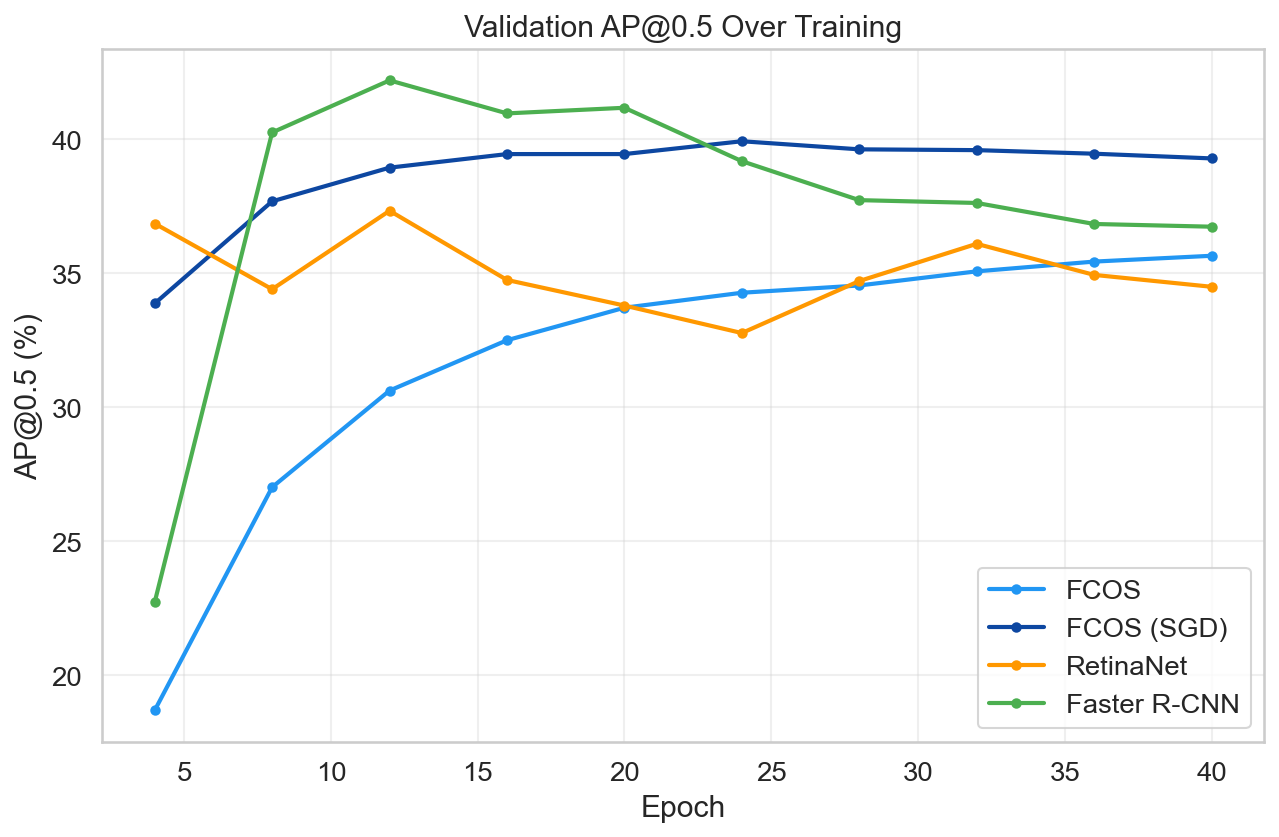
\includegraphics[height=0.30\textheight]{val_ap_over_epochs.png}
\end{frame}

%------------------------------------------------------------------------------
\begin{frame}{Metrics}
  \small
  \begin{columns}[T]
    \column{0.5\textwidth}
      \textbf{Detection}
      \begin{itemize}\small
        \item \hl{AP@0.5} (101-point, COCO): headline.
        \item Size-stratified AP on \emph{RSNA} tertiles (COCO buckets are degenerate here).
        \item $AR_{10}$: recall at 10 detections/image.
      \end{itemize}
    \column{0.5\textwidth}
      \textbf{Patient-level}
      \begin{itemize}\small
        \item F1 at threshold $\tau$ (paper uses $\tau=0.3$).
        \item \hl{ROC AUC}: threshold-free, calibration-insensitive.
        \item \hl{FROC/CPM}, \hl{ECE} (calibration).
      \end{itemize}
  \end{columns}
  \vspace{0.6em}
  \begin{block}{\small Why so many metrics?}
    \small Because a single fixed-threshold number can be dominated by \hl{score calibration}
    rather than detection quality, the central subtlety of our results.
  \end{block}
\end{frame}

%------------------------------------------------------------------------------
\begin{frame}{Results: Detection Performance}
  \centering\footnotesize
  \begin{tabular}{lccc}
    \toprule
    Method & AP@0.5 [95\% CI] & ROC AUC & note \\
    \midrule
    FCOS (Adam) & 35.3 [32.6, 38.4] & 86.5 & optimiser-faithful \\
    FCOS (SGD, our ablation) & 39.8 [37.1, 43.1] & 88.1 & \\
    RetinaNet & 41.2 [38.2, 44.1] & 89.1 & \\
    \textbf{Faster R-CNN} & \textbf{42.9} [40.0, 46.3] & 88.9 & \textbf{our best} \\
    Ensemble (FCOS+Retina, WBF) & 42.0 [39.2, 45.6] & 87.5 & \\
    \midrule
    \textit{Wu et al.\, FCOS} & \textit{48.6} & -- & \textit{their eval} \\
    \textit{Wu et al.\, proposed} & \textit{51.5} & -- & \textit{their eval} \\
    \bottomrule
  \end{tabular}
  \vspace{0.5em}
  \begin{itemize}\small
    \item In \emph{our} controlled setup: \hl{anchor-based $>$ anchor-free} (Faster R-CNN, RetinaNet
      top FCOS), the \hl{reverse} of the paper's ordering.
    \item ROC AUC lies in a \hl{tight 86.5--89.1\%} band: true ranking quality is similar.
  \end{itemize}
\end{frame}

%------------------------------------------------------------------------------
\begin{frame}{The Honest Paper Comparison}
  \small
  \begin{alertblock}{\small We do NOT beat the paper's absolute numbers, and we say so}
    \small Our best is 42.9; the paper reports FCOS 48.6 and 51.5 for its method.
  \end{alertblock}
  \textbf{Why? An evaluation gap, not a training gap:}
  \begin{itemize}\small
    \item Our recipe is if anything \emph{stronger} (EMA, mixed precision, medical augmentation).
    \item But the paper's recall is far higher: $\mathrm{AR}_{10}\approx\hl{96\text{--}99}$ vs.\ our
      $\approx\hl{85}$. Higher recall at fixed IoU \hl{inflates AP}, regardless of paradigm.
    \item No code, weights or split released $\Rightarrow$ protocols cannot be aligned.
  \end{itemize}
  \begin{block}{\small The defensible claim}
    \small The only protocol-matched comparison is the \hl{internal} one, and there the
    paradigm ordering \hl{reverses} relative to the paper. That is our contribution.
  \end{block}
\end{frame}

%------------------------------------------------------------------------------
\begin{frame}{The Calibration Artefact (our strongest result)}
  \small
  At fixed $\tau=0.3$, the WBF ensemble ``wins'' patient F1 ($63.0\%$, $+13.5$).
  \textbf{But this is a calibration artefact:}
  \begin{itemize}\small
    \item Detectors' optimal thresholds differ wildly (FCOS 0.47, RetinaNet 0.13, F-RCNN 0.82);
      a fixed cut penalises \hl{mis-calibrated} models, not worse models.
    \item Under a \emph{fair} operating point (Youden on a held-out half, or a learnt 5-fold
      aggregator) the ensemble edge shrinks to $\le\!1$ F1 and is \hl{overtaken by RetinaNet}
      (learnt-aggregator F1 \hl{67.3\%}, best in the study).
  \end{itemize}
  \vspace{0.2em}
  \centering
  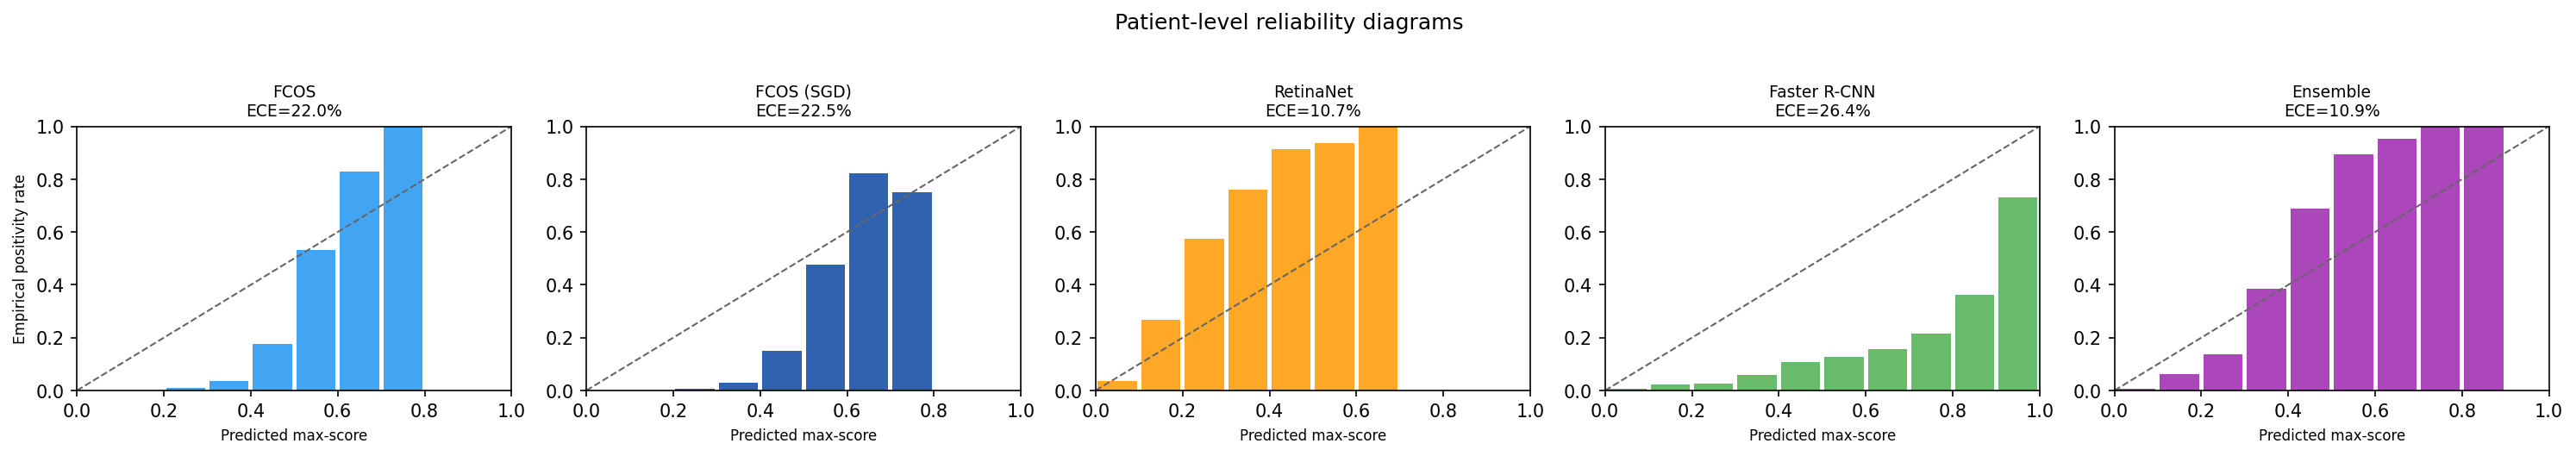
\includegraphics[width=0.92\textwidth]{calibration.png}\\
  {\scriptsize Reliability diagrams (predicted confidence vs.\ empirical positivity); ECE above each panel.}
\end{frame}

%------------------------------------------------------------------------------
\begin{frame}{Robustness Checks (no extra training)}
  \begin{columns}[T]
    \column{0.5\textwidth}
      \small
      All run on cached predictions:
      \begin{itemize}\small
        \item Patient-level \hl{bootstrap CIs} on AP@0.5.
        \item Three-way split for the threshold.
        \item RSNA-percentile size buckets.
        \item FROC/CPM, reliability/ECE.
        \item Learnt 5-fold patient aggregator.
        \item \hl{Paired bootstraps} on AP differences.
      \end{itemize}
      \vspace{0.3em}
      {\footnotesize Only Faster R-CNN strictly beats another detector
      ($-3.07$ vs.\ FCOS-SGD, $p<0.001$); the ensemble does \emph{not} beat RetinaNet
      ($+0.88$, $p=0.25$).}
    \column{0.5\textwidth}
      \centering
      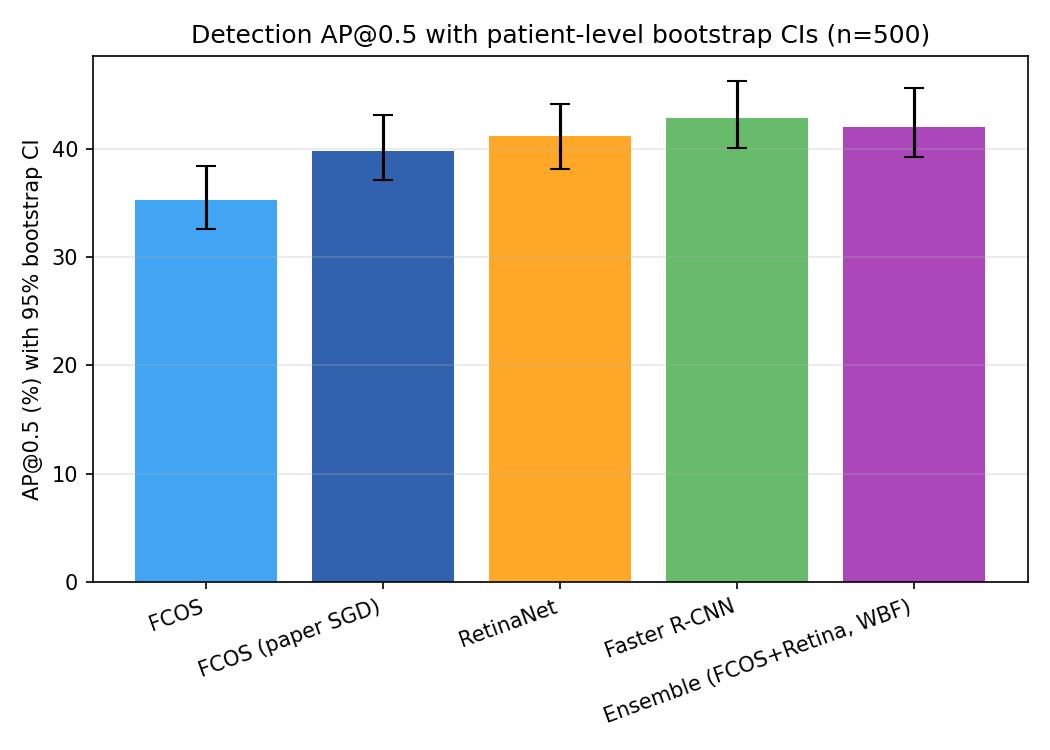
\includegraphics[height=0.62\textheight]{ap_bootstrap.png}
  \end{columns}
\end{frame}

%------------------------------------------------------------------------------
\begin{frame}{Limitations (stated up front)}
  \small
  \begin{itemize}\setlength\itemsep{0.5em}
    \item \hl{Single training seed} per detector: run-to-run variance ($\pm1$--$2$ AP) is not
      captured $\Rightarrow$ we treat AP differences $<\!2$ points as unresolved.
    \item \hl{No held-out test set}: the same split is used for selection, thresholds and CIs
      (selection-on-val bias).
    \item \hl{Asymmetric ablation}: SGD tried only on FCOS $\Rightarrow$ paradigm vs.\ optimiser
      separated on the FCOS side only.
    \item No per-site stratification, no external dataset; cross-paper AP not directly comparable.
  \end{itemize}
  \vspace{0.4em}
  \begin{block}{\small}
    \small Disclosing these \emph{before} being asked is the point: rigour and honesty over a
    polished-but-fragile headline.
  \end{block}
\end{frame}

%------------------------------------------------------------------------------
\begin{frame}{Conclusion}
  \small
  \begin{enumerate}\setlength\itemsep{0.45em}
    \item Under a \hl{shared backbone, recipe and evaluation}, anchor-based detectors beat
      anchor-free FCOS on AP@0.5, the \hl{reverse} of the paper's paradigm claim.
    \item We do \emph{not} reproduce the paper's absolute numbers; the gap is one of
      \hl{evaluation} (recall $\sim$96--99 vs.\ 85), not training.
    \item The ensemble's patient-level ``win'' is a \hl{calibration artefact}: at a fair operating
      point RetinaNet is the best single model (F1 67.3\%).
    \item The numerical-analysis backbone (EMA filter, focal gradient, GIoU, cosine, bootstrap)
      justifies every training choice.
  \end{enumerate}
  \vfill
  \centering
  \textbf{\textcolor{polimi}{The contribution is a fair, honest, statistically grounded comparison.}}
\end{frame}

%------------------------------------------------------------------------------
\begin{frame}[plain]
  \centering
  \vfill
  {\Large\textcolor{polimi}{\textbf{Thank you}}}\\[0.5em]
  {\small Questions?}\\[1.2em]
  
\includegraphics[height=1.2cm]{logo_polimi.png}\\[0.6em]
  {\footnotesize Code: \texttt{github.com/moa155/pneumonia-detection-naml}}
  \vfill
\end{frame}

\end{document}
